%%%%%%%%%%%%%%%%%%%%%%%%%%%%%%%%%%%%%%%%%%%%%%%%%%%%%%%%%%%%%%%%%%%%%%%%%%%%%%%%
%2345678901234567890123456789012345678901234567890123456789012345678901234567890
%        1         2         3         4         5         6         7         8

\documentclass[letterpaper, 10 pt, conference]{ieeeconf}  % Comment this line out if you need a4paper

%\documentclass[a4paper, 10pt, conference]{ieeeconf}      % Use this line for a4 paper

\IEEEoverridecommandlockouts                              % This command is only needed if
                                                          % you want to use the \thanks command

\overrideIEEEmargins                                      % Needed to meet printer requirements.

%In case you encounter the following error:
%Error 1010 The PDF file may be corrupt (unable to open PDF file) OR
%Error 1000 An error occurred while parsing a contents stream. Unable to analyze the PDF file.
%This is a known problem with pdfLaTeX conversion filter. The file cannot be opened with acrobat reader
%Please use one of the alternatives below to circumvent this error by uncommenting one or the other
%\pdfobjcompresslevel=0
%\pdfminorversion=4

% See the \addtolength command later in the file to balance the column lengths
% on the last page of the document

% The following packages can be found on http:\\www.ctan.org
%\usepackage{graphics} % for pdf, bitmapped graphics files
%\usepackage{epsfig} % for postscript graphics files
%\usepackage{mathptmx} % assumes new font selection scheme installed
%\usepackage{times} % assumes new font selection scheme installed
\usepackage{amsmath} % assumes amsmath package installed
\usepackage{amssymb}  % assumes amsmath package installed
\usepackage{balance}
\usepackage{xspace}
\usepackage{csquotes}
\usepackage{hyperref}
\usepackage{stmaryrd}
\usepackage{cite}
\usepackage[svgnames,dvipsnames]{xcolor}
\definecolor{shadeGray}{rgb}{0.9,0.95,0.95}
\usepackage[bordercolor=red, backgroundcolor=shadeGray, linecolor=red, textwidth=0.8in, textsize=footnotesize]{todonotes}
\usepackage{listings}
\usepackage{tikz}
\usepackage{pgfplots}
\usepackage{subfig}
\usepackage{paralist}
\lstdefinestyle{corelang}{
  %frame=tb,
  %rulesepcolor=\color{gray},
  rulecolor=\color{gray},
  morekeywords={
  repeat, times, foreach, visit, pick, drop, containing, avoiding, while, strict,
  move, right, move, left, in, every, has, color, shape, possible, if, at, and, or, minus, not
  },%in,
  keywordstyle=[2]\emph,
  keywords=[2]{world, point, robot, item, red, blue, yellow, green, triangle, square, circle},
  sensitive=true,
  morecomment=[l]{//},
  morecomment=[s]{/*}{*/},
  commentstyle=\color{gray},
  showstringspaces=false,
  %columns=fullflexible,
  mathescape=true,
  numberstyle=\tiny,
  basicstyle=\footnotesize\ttfamily,
  numbersep=5pt,
  stepnumber=2,
  numbers=none,                   % where to put the line-numbers
  morestring=[b]"
}
\lstset{style=corelang}
\usepackage[T1]{fontenc}  % this is necessary for beramo to work
\usepackage[scaled=0.80]{beramono}  % our monospace font
\allowdisplaybreaks

\def\pick{\mathtt{pick}}
\def\drop{\mathtt{drop}}
\def\visit{\mathtt{visit}}
\def\avoiding{\mathtt{avoiding}}
\def\while{\mathtt{while}}

\let\proof\relax    % there is an option clash with amsthm with something in IEEEconf
\let\endproof\relax
\usepackage{amsthm}
\usepackage{thmtools}
\declaretheorem[style=definition,qed=$\blacksquare$]{example}

\newcommand{\tool}{Flipper\xspace}

\newcommand{\sem}[2]{\llbracket \texttt{#1}\rrbracket &::= #2}
\newcommand{\bbraces}[1]{\llbracket \texttt{#1}\rrbracket}
\newcommand{\until}[2]{#1\; \mathcal{U}\; #2}

\title{\LARGE \bf Precise but Natural Specifications for Robot Tasks
}


\author{Brendon Boldt$^1$\quad Ivan Gavran$^2$ \quad Eva Darulova$^2$ \quad Rupak Majumdar$^2$%
\thanks{
$^1$Marist College, USA,
$^2$Max Planck Institute for Software Systems, Germany
}%
\thanks{Brendon Boldt was supported by a DAAD RISE Internship.}
}
% \author{Albert Author$^{1}$ and Bernard D. Researcher$^{2}$% <-this % stops a space
% \thanks{*This work was not supported by any organization}% <-this % stops a space
% \thanks{$^{1}$Albert Author is with Faculty of Electrical Engineering, Mathematics and Computer Science,
%         University of Twente, 7500 AE Enschede, The Netherlands
%         {\tt\small albert.author@papercept.net}}%
% \thanks{$^{2}$Bernard D. Researcheris with the Department of Electrical Engineering, Wright State University,
%         Dayton, OH 45435, USA
%         {\tt\small b.d.researcher@ieee.org}}%
% }


\begin{document}



\maketitle
\thispagestyle{empty}
\pagestyle{empty}


%%%%%%%%%%%%%%%%%%%%%%%%%%%%%%%%%%%%%%%%%%%%%%%%%%%%%%%%%%%%%%%%%%%%%%%%%%%%%%%%
\begin{abstract}
We present \tool, a
% community-powered
natural language interface for describing
high level task specifications for robots
that are compiled into robot actions.
\tool starts with a formal core language for task planning that allows
expressing rich temporal specifications and
uses a semantic parser to provide a natural language interface.
\tool provides immediate visual feedback by executing an automatically
constructed plan of the task in a graphical user interface.
This allows the user to resolve potentially ambiguous interpretations.
\tool extends itself via \emph{naturalization}: users of \tool can
define new commands, which are generalized and added as new rules to the core language,
gradually growing a more and more natural task specification language.
%
Unlike other task-specification systems, \tool enables natural language
interactions while maintaining the expressive power and formal precision of a programming language.
We show through an initial user study that natural language interactions and generalization
can considerably ease the description of tasks.
Moreover, over time, users employ more and more concepts outside of the initial core language.
Such extensions are available to the \tool community, and users can use concepts that others have defined.

\end{abstract}


%%%%%%%%%%%%%%%%%%%%%%%%%%%%%%%%%%%%%%%%%%%%%%%%%%%%%%%%%%%%%%%%%%%%%%%%%%%%%%%%

\section{Introduction}


\subsection{Architecture}

The architecture of \tool has four main components.
The first is a core language to express temporal objectives
in the world.
The second is a semantic parser to map natural language
utterances to representations in the core language.
The third is a planner that, given a goal in the core language,
generates a plan for the robot to execute the goal if possible.
Finally, a visual user interface provides the user real-time
feedback by exhibiting the effect of a plan in a simulated environment. 



\section{Core Language}
Interesting core-language examples

\begin{itemize}
	\item drop an item to any field that contains both red item and circle-shaped item (can be the same item): \textit{foreach point in \{world containing item has color red\} and \{world containing item has shape circle\} \{visit point; drop item\}}
	\item if possible, form a horizontal line on the floor out of all items robot currently has and starting at robot's current position: \textit{strict \{while robot has item \{drop item; move right\}\}; strict \{while robot has item \{drop item; move left\}\}}
	\item keep bringing circle-shaped items to room1 until there is a red item in room1: \textit{while not \{ item has color red at room1\} \{visit \{world containing item has shape circle\} minus room1; pick item has shape circle; visit room1; drop item has shape circle\}}

\end{itemize}

\section{Naturalization of the Language}

The task of putting all items of different colors to different rooms looks in the core language like this \\
\begin{displayquote}
 \textit{foreach point in world containing item has color red \{ visit point; pick every item has color red\}; visit room1; drop every item has color red; foreach point in world containing item has color green \{ visit point; pick every item has color green\}; visit room2; drop every item has color green; foreach point in world containing item has color blue \{ visit point; pick every item has color blue\}; visit room3; drop every item has color blue; foreach point in world containing item has color yellow \{ visit point; pick every item has color yellow\}; visit room4; drop every item has color yellow} 
\end{displayquote} 
 The same task could be accomplished using naturalization with 
\begin{displayquote} 
 \textit{red to room1; green to room2; blue to room3; yellow to room4}
\end{displayquote} 
  with a single definition of \textit{red to room1} as
  \begin{displayquote}
  \textit{foreach point in world containing item has color red \{ visit point; pick every item has color red\}; visit room1; drop every item has color red}
  \end{displayquote}.
  If the next thing would be to put all items of different shapes to different rooms, it would again be possible to do it by 
\begin{displayquote}  
   \textit{ triangle to room1; circle to room2; square to room3}
   \end{displayquote}
\section{Evaluation}

\tool is available at \url{flipper.mpi-sws.org}. It consists of a backend
responsible for semantic parsing, a frontend that visually demonstrates to the user the effect of each interpretation of an utterance (both based on \cite{wangVoxelurn}), and a planning module.
%\footnote{The code is available at \url{github/gitlab for both repositories}}.
As our core language is a mixture of concepts typical for
imperative programming (e.g.\ \lstinline{move left}) and an \textit{avoid-until-
reach} temporal specification, we use an adapted version of the
$A^*$~\cite{hipsterHeuristicPlanner} algorithm as our planner. 
% Depending on a deployment scenario and language requirements, we could choose a different
% planner supporting declarative specifications~\cite{metricFF,hadasLTLMop,antlab}.

\subsection{Goal of Evaluation}
Our final goal is to create a system which people with different levels of
proficiency in the core language would use. Envisioned users range from
\emph{expert users}, i.e., those that define new commands to make the
communication with the robot simpler, all the way to those who do not know the
language at all. The latter take advantage of commands that \emph{sound as if they
should work}, and which were defined by other users of the system.

In the evaluation we were thus interested in two properties:
\begin{enumerate}
	\item whether or not users are inclined to define new commands and whether
		those commands make their work easier, and
	\item how much they are able to benefit from other people's definitions
		(without knowing them in advance).
\end{enumerate}
The first property corresponds to the ability to define functions in a programming language,
except that \tool generalizes definitions from examples. The second property
describes how much closer the system gets to pure natural-language interface if
there is a number of active expert users. We thus want to test our intuition
that different people use similar linguistic expressions for similar commands
and that is why they do not have to be aware of existing definitions.

\subsection{Setup}
We created a list of 21 tasks. The tasks levels ranged from easy (e.g.
``get one green square'') to difficult (e.g. ''bring all red items to a
room that contains a yellow square''). The list of all tasks, as well as
all our experimental data is available at \tool's website.
% \todo[inline]{@Ivan: reminder to put list of tasks on website}
%
We recruited thirteen participants, all with prior programming experience but without any
knowledge of the system, and split them into three groups:
\begin{itemize}
	\item Group $A$ (4 members) was only allowed to use the core language,

	\item Group $B$ (6 members) could additionally define their own concepts,

	\item Group $C$ (3 members) additionally had access to concepts defined by two
		expert users (familiar with the system and the language) as well as by other
		participants from group C in real time.
\end{itemize}
%
At the start of the experiment, each group had 30 minutes to familiarize themselves with the core language by following a tutorial. 
%\footnote{tutorial is available at \url{TUTORIALURL}}.
Then participants were instructed to solve the 21 tasks as they saw fit, i.e., not necessarily in the most general way.
The average time needed to solve all tasks was 90 minutes (no deadline was set). 
For each participant, we measured the number of accepted commands, i.e., the syntactically 
correct ones coming either from the core or the induced language,
and the total number of words, defined concepts, and induced commands used to finish all tasks. 
For induced commands we additionally distinguish whether they were defined by the same or by another participant.

%\paragraph*{\textbf{Difficulty of Learning the Core Language}}

Learning any new programming language in half an hour is a nontrivial task. In
our experiment, the average number of successfully parsed queries in group $A$
(only using the core language) was 75\%, with some differences between
the participants (63\%, 70\%, 77\% and 90\%).


\subsection{Results}

\paragraph*{\textbf{Usefulness of Naturalization}}
To assess the usefulness of naturalization, we compare the total number of
tokens needed to finish the tasks for the different groups
(\autoref{fig:numTokens}), and how often participants in groups $B$ and $C$ used
defined concepts (\autoref{fig:groupBAndCCoreVsInduced}).
The latter shows that participants who were allowed to define their own concepts
also used that opportunity.
When comparing the participants from groups $B$ and $C$ to those of group $A$, 
it is clear that the participants who were able to use naturalization end up with less work in 
terms of total number of tokens needed to finish the tasks. 
Specifically, the average number of tokens needed for groups $B$ and $C$ is 1156, 
while for group $A$ it is 1765. 
This takes into account all tokens, also the ones from unsuccessful commands. 
We include these, as some number of unsuccessful commands by groups that use naturalization comes from trying 
out commands they believed might be defined by others.
Only considering successful commands, groups $B$ and $C$ use in total 738 tokens compared to 1287 in group $A$, 
i.e., an improvement of 43\% with respect to the usage of the core language only.
These results suggest that naturalization reduces users' effort. 
It is important to note that individual performances of participants within a single group vary, as shown in~\autoref{fig:numTokens}.

\paragraph*{\textbf{Naturalization across Users}}
Participants in group $C$ had access to the concepts defined by others. Interestingly, these
participants adopted different strategies. While they were on average more likely to use induced
language than the core language (43 vs.\ 35 commands), only one participant relied primarily on the induced language.
The other two users used slightly more core than induced language (see~\autoref{fig:groupBAndCCoreVsInduced}).
The main point of the experiment for group $C$ was to see whether the existence of previously defined concepts is helpful.
We first notice that participants were indeed using concepts defined by others (\autoref{fig:groupCRulesInducedBySelfVsOthers}). 
Again, the numbers differ among participants. 
By looking closer at the kinds of commands issued by each participant, we see that these differences 
stem from their individual styles: participant $C2$ chose to try small building blocks that matched the style of 
the two expert users whose definitions were available to group $C$. 
Participant $C3$, on the other hand, used commands similar to the core language.
%\footnote{All commands by all experiment participants are available at \url{URLFORALLDATA}}.
Curiously, after the experiment two participants (C1 and C3) claimed that they have not much used the predefined rules 
and that they ended up using almost exclusively self-defined concepts (in addition to the the core language). 
The data, however, told a different story (\autoref{fig:groupCRulesInducedBySelfVsOthers}): $C1$ roughly equally used rules defined by others and by himself, while $C3$ 
used much more induced rules. 
Upon inspection of the logs, it turned out that on many occasions they believed they were using the core language, while in fact they used induced concepts
defined by others
(e.g. \lstinline{move 2 right} or \lstinline{drop all blue items}).

\paragraph*{\textbf{Types of Defined Concepts}}
Upon closer inspection of the concepts the participants defined, we see that a majority falls into two categories:
\begin{inparaenum}[(1)]
\item simplifying individual commands and
\item defining functions.
\end{inparaenum}
%
Examples for the first case are
\lstinline{pick green square} defined as \lstinline{pick item has color green} and
\lstinline{visit empty space} defined as \lstinline$visit world minus {world containing item}$.

For the second case a simple example is
\lstinline{visit both triangle and green} defined as
\begin{lstlisting}
visit { {world containing item has shape triangle} and
  {world containing item has color green} }
\end{lstlisting}
There were also function definitions that involved previous function definitions,
such as \lstinline{line red} being defined as
\lstinline$fetch all red; while {robot has item} {drop item; move left}$.
Another noticeable phenomenon was that group C had to define some concepts already defined by others.
The reason was small variations in the utterances (e.g. \lstinline{pick red} vs.\
\lstinline{take a red} vs.\ \lstinline{take a red item}) which can be caught by a more
comprehensive natural language processing module.


\begin{figure}[t!]

		\resizebox{\linewidth}{!}{
		\centering
				\begin{tikzpicture}
				\begin{axis}[
				ticklabel style = {font=\tiny},
				    ybar,
				    bar width = 3,
				    area legend,
				    %enlargelimits=0.15,
				    legend style={at={(0.5,-0.15)},
				      anchor=north,legend columns=-1},
				    ylabel={\# tokens},
				    symbolic x coords={A1, A2, A3, A4, B1,B2,B3,B4,B5,B6,C1,C2,C3},
				    xtick=data,
	%			    nodes near coords,
				    ]
				\addplot coordinates {(A1,1105 ) (A2,1035 ) (A3,1853) (A4, 1156) (B1, 375) (B2, 957) (B3, 549) (B4, 1063) (B5, 970) (B6, 985) (C1,649) (C2,622) (C3,478)};
				\addplot coordinates {(A1,1398 ) (A2,1220 ) (A3,2790) (A4, 1654) (B1, 760) (B2,1364) (B3, 822) (B4, 1471) (B5, 1578) (B6, 1270) (C1,1098) (C2,982) (C3,1061)};
			%	\addplot coordinates {(B1,30) (B2, 61) (B3, 29) (B4, 107) (B5, 80) (B6, 158) (C1,46) (C2,13) (C3,48)};
				\legend{successful commands, all commands}
				\end{axis}
				\end{tikzpicture}
	}
	\caption{Total number of tokens used per participant}
	\label{fig:numTokens}
	\end{figure}






\begin{figure}[t!]
		\resizebox{\linewidth}{!}{
		\centering



				\begin{tikzpicture}
				\begin{axis}[
				    ybar,
				    bar width = 5,
				    area legend,
				    %enlargelimits=0.15,
				    legend style={at={(0.5,-0.15)},
				      anchor=north,legend columns=-1},
				    ylabel={\# commands},
				    symbolic x coords={B1,B2,B3,B4,B5,B6,C1,C2,C3},
				    xtick=data,
	%			    nodes near coords,
				    ]
				\addplot coordinates {(B1, 38) (B2, 64) (B3, 47) (B4, 6) (B5, 45) (B6, 62) (C1,37) (C2,65) (C3,28)};
				\addplot coordinates {(B1,30) (B2, 61) (B3, 29) (B4, 107) (B5, 80) (B6, 158) (C1,46) (C2,13) (C3,48)};
				\legend{induced, core}
				\end{axis}
				\end{tikzpicture}


	}

	\caption{Core-language commands vs induced commands for groups B and C}
	\label{fig:groupBAndCCoreVsInduced}
	\end{figure}


\begin{figure}[t!]
	\resizebox{\linewidth}{!}{
		\centering
		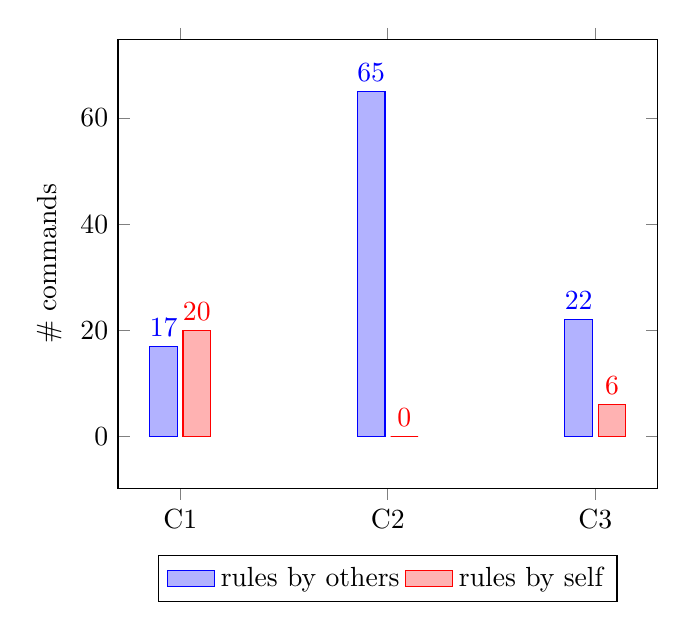
\begin{tikzpicture}
			\begin{axis}[
			    ybar,
			    area legend,
			    enlargelimits=0.15,
			    legend style={at={(0.5,-0.15)},
			      anchor=north,legend columns=-1},
			    ylabel={\# commands},
			    symbolic x coords={C1,C2,C3},
			    xtick=data,
			    nodes near coords,
			    ]
				\addplot coordinates {(C1,17) (C2,65) (C3,22)};
				\addplot coordinates {(C1,20) (C2,0) (C3,6)};
				\legend{rules by others, rules by self}
			\end{axis}
		\end{tikzpicture}
	}
	\caption{Using rules induced by others vs. self-induced rules}
	\label{fig:groupCRulesInducedBySelfVsOthers}
\end{figure}


%\begin{figure}[t!]
%		%\resizebox{\linewidth}{!}{
%		\centering
%		\subfloat[][Core language commands vs induced commands]{\resizebox{0.5\linewidth}{!}{
%
%				\label{fig:groupCCoreVSInduced}
%				\begin{tikzpicture}
%				\begin{axis}[
%				    ybar,
%				    area legend,
%				    enlargelimits=0.15,
%				    legend style={at={(0.5,-0.15)},
%				      anchor=north,legend columns=-1},
%				    ylabel={\# commands},
%				    symbolic x coords={C1,C2,C3},
%				    xtick=data,
%				    nodes near coords,
%				    ]
%				\addplot coordinates {(C1,37) (C2,65) (C3,28)};
%				\addplot coordinates {(C1,46) (C2,13) (C3,48)};
%				\legend{induced, core}
%				\end{axis}
%				\end{tikzpicture}
%
%	}
%			}
%\subfloat[][Using rules induced by others vs. self-induced rules]{\resizebox{0.5\linewidth}{!}{
%
%				\label{fig:groupCRulesInducedBySelfVsOthers}
%				\begin{tikzpicture}
%				\begin{axis}[
%				    ybar,
%				    area legend,
%				    enlargelimits=0.15,
%				    legend style={at={(0.5,-0.15)},
%				      anchor=north,legend columns=-1},
%				    ylabel={\# commands},
%				    symbolic x coords={C1,C2,C3},
%				    xtick=data,
%				    nodes near coords,
%				    ]
%				\addplot coordinates {(C1,17) (C2,65) (C3,22)};
%				\addplot coordinates {(C1,20) (C2,0) (C3,6)};
%				\legend{rules by others, rules by self}
%				\end{axis}
%				\end{tikzpicture}
%
%	}
%			}
%	\caption{Usage of induced rules in group C}
%
%\end{figure}

\section{Related work}

There are many systems commanding or communicating naturally with robots as well as creating programming
languages for robots usable by non-programmers, starting with the seminal work in SHRDLU~\cite{shrdlu},
and continuing over the years~\cite{kollarDialog,thomasonDialog,roboFlow}.
% We believe that natural language---if done right---is the most promising interface with robots (or machines in general).
% \todo[inline]{ED: maybe too strong? perhaps just say, it's an alternative?}
% Kollar et al.~\cite{kollarDialog} and Thomason et al.~\cite{thomasonDialog} recognize the
% need for a dialog between a robot and a human in order for the robot to
% understand the human's intentions and to build trust in mutual understanding.
For example, Thomason et al.~\cite{thomasonDialog} demonstrate a system in which
utterances are mapped to $\lambda$-calculus computations and the robot 
fills in the gaps in a simple \textit{action-patient-recipient} pattern, supporting
navigation and delivery.
%
%  whereas \tool's robot actions can be of arbitrary complexity.
%\todo[inline]{ED: how is SHRDLU related to the other works? I would skip the
%sentence about the need for trust. Sounds subjective to me.}
%\todo[inline]{ED: what is an action-patient-recipient pattern? Is there a different
%word for patient?}
%\todo[inline]{IG: it is a type of thematic relation, a concept from linguistics. At least two papers from our related work are using this term}
%Alexandrova et al.\cite{roboFlow} created a flow-based visual programming language, balancing
%intuitiveness and expressivity. 

Formal and logical languages for planning have a long research tradition in AI and formal methods.
Recently, the work by Kress-Gazit et
al.~\cite{hadasTranslatingStructuredEnglish,hadasLTLMop,
hadasProvablyCorrectReactiveControlFromNaturalLanguage} focuses on translating
natural language into linear temporal logic to bridge the gap from users to formal methods
tools.
One project uses a pipeline of general-purpose NLP 
methods~\cite{hadasProvablyCorrectReactiveControlFromNaturalLanguage}, with VerbNet~\cite{schulerVerbnet}
at the core of semantic interpretation. A robot is additionally able
to give an answer to what it is currently doing, based on the natural language
to LTL translation tree, as well as to explain why an action is unrealizable. A
limitation is, however, that the set of actions a robot can perform is still
restricted to implemented semantic behaviours. On the other hand,~\cite{hadasTranslatingStructuredEnglish}
can process any (GR(1)) LTL specification, but the burden is on the human to use
only \emph{structured English}. \tool accomplishes both, with the tradeoff 
that at least some of the users are able to learn the core language.

Tellex et al.~\cite{tellexGrounding} solve the problem of grounding utterances
from the command to objects in space by introducing a hierarchical structure
that connects expressions such as \emph{beside the truck} and \emph{beside the
box}. Paul et al.~\cite{paulGrounding} solve the same problem, but support
abstract expressions such as \emph{first cube in the second row}. This line of
work is connected to the one described in the previous paragraph in the work by
Boteanu et al.~\cite{boteanuVerifiableGrounding}---there the grounding
problem is put in the context of reactive temporal commands. In this line of
work, unlike in \tool, the robot cannot be taught new concepts. On the other hand,
\tool does not support talking about abstract spatial relations between items
in its world. To support this, \tool's core language would need to be modified
(and one could then use the mentioned techniques).

\tool is inspired by and based upon the work on naturalization of formal
languages by Wang et al.~\cite{wangVoxelurn}, which considers
a block world where a user can build various shapes of different
colors. The application of naturalization to a robot world introduces new
challenges: the language contains declarative and unrealizable
commands and dynamic behavior that changes the state of the world.
A similar approach of learning the language from users is presented in~\cite{azariaLia}, but in the context of personal
assistants. 
Iyer et al.~\cite{iyerLearningNeuralSemanticParser} use user's feedback to 
minimize the effort needed for additional annotation of data and iteratively improve their semantic parser 
that translates natural language utterances to SQL queries. 
Beltagy and Quirk~\cite{beltagyIFTT} train a model (an ensemble of a neural network and logistic
regression) that translates a task description from an IFTTT dataset into
executable representations. They show several ways to improve the performance, the
most interesting of which is creating synthetic data by paraphrasing task
descriptions. Work by Lin et al.~\cite{linTelina} has a similar motivation:
starting with questions from popular programming-help websites that describe
programmers' intentions, they devise bash one-liners accomplishing it. 
This kind of work enables semantic parsing from 
less direct instructions, but is not easily adaptable to users interactively giving clues to the 
system about the meaning of the utterance.
None of these papers targeted the robotics domain.


\section{Conclusion}

% Effectively communicating with robots has been a long-standing research problem.
We have shown that naturalizing a domain-specific programming language is well suited
to provide a natural language interface to robot task specifications.
\tool provides the precision, expressivity, and extensibility of a programming
language, while ensuring a natural experience for humans.
\tool adapts its language to its users by learning new concepts from them. 
The results of our initial evaluation are encouraging and suggest
that a formal language for instructing robots can be turned with community
effort into a \emph{domain specific natural language}.

To accomplish our goal to its full extent, a few challenges remain to be solved.
The first one is lowering the entry bar to the system in its early phase, i.e.
learning the core language.
This could be accomplished by adding syntactic sugar or a specialized interface,
while keeping the rich formalism as a latent representation of
the space of robot tasks.
% A second direction is to include more sophisticated NLP techniques on top of the
% naturalization process such as lemmatization, rephrasing of definition heads, and
% rephrasing of the initial formal language.
Finally, the user experience of \tool can be improved to offer explanations for
unparseable utterances, better depict alternate interpretations of an utterance
which have the same execution, or auto-complete for available pre-defined concepts.


\balance
% \addtolength{\textheight}{-12cm}   % This command serves to balance the column lengths
                                  % on the last page of the document manually. It shortens
                                  % the textheight of the last page by a suitable amount.
                                  % This command does not take effect until the next page
                                  % so it should come on the page before the last. Make
                                  % sure that you do not shorten the textheight too much.

%%%%%%%%%%%%%%%%%%%%%%%%%%%%%%%%%%%%%%%%%%%%%%%%%%%%%%%%%%%%%%%%%%%%%%%%%%%%%%%%



%%%%%%%%%%%%%%%%%%%%%%%%%%%%%%%%%%%%%%%%%%%%%%%%%%%%%%%%%%%%%%%%%%%%%%%%%%%%%%%%



%%%%%%%%%%%%%%%%%%%%%%%%%%%%%%%%%%%%%%%%%%%%%%%%%%%%%%%%%%%%%%%%%%%%%%%%%%%%%%%%



%%%%%%%%%%%%%%%%%%%%%%%%%%%%%%%%%%%%%%%%%%%%%%%%%%%%%%%%%%%%%%%%%%%%%%%%%%%%%%%%



\bibliography{relatedWorkList}
\bibliographystyle{ieeetr}



\end{document}
